\documentclass[a4paper,12pt]{article}

\usepackage[utf8x]{inputenc}
\usepackage[english, russian]{babel}

\usepackage{tabularx}
\usepackage{multirow}
\usepackage{graphicx}

\usepackage{diagbox}

\usepackage{makecell}
\usepackage{indentfirst}


\usepackage{textcomp}

\usepackage{fullpage}

\usepackage{amsmath}
\usepackage{amsfonts}
\usepackage{amssymb}

\exhyphenpenalty=10000
\doublehyphendemerits=10000
\finalhyphendemerits=5000

\begin{document}

\begin{titlepage}
\newpage

\

\begin{center}
	\large		
   	Министерство образования и науки Российской Федерации\\[0.5cm]
    	
	ФГБОУ ВО Рыбинский государственный авиационный технический университет имени П.А. Соловьева\\[1.0cm]

	Факультет радиоэлектроники и информатики\\[0.25cm]
		
	Кафедра математического и программного обеспечения\\ электронных вычислительных средств\\[1.5cm]

	\Large
	\textbf{\textsc{ОТЧЕТ ПО ЛАБОРАТОРНОЙ РАБОТЕ }}\\[0.25cm]
	по  дисциплине\\
	\textbf{Математические методы анализа данных}\\[0.5cm]
	
	по теме\\
	Кластерный анализ

\end{center}

\vfill	
\begin{tabularx}{0.95\textwidth}{lXr}
Студент группы ИПБ-13 			& &	Иванов Р.А.\\
Преподаватель, доцент	& & Воробьев К. А.\\
\end{tabularx}

\vspace{1.5cm}
\center Рыбинск 2017
\end{titlepage}	


\newpage
\setcounter{page}{2}

\tableofcontents

\newpage\section{Исходные данные}
В качестве исходных данных для выполнения класстерного анализа были сгенериррованы на плоскости 50 точек с координатами в диапазоне от (0,0) до (3,8), значение каждой координаты было получено на основе генератора случайных чисел с равномерным распределением(рис. ~\ref{fig:im_0}).

\begin{center}
	\begin{figure}[h]
	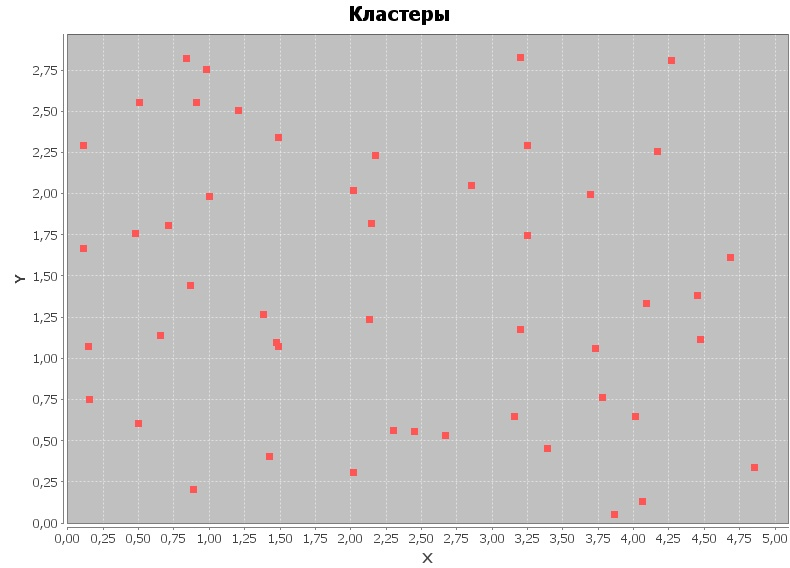
\includegraphics[scale=0.8]{figure_0.png}
	\caption{Исходные данные}
	\label{fig:im_0}
	\end{figure}
\end{center}

\newpage\section{Задача кластерного анализа}
Кластерный анализ выполняет следующие основные задачи:
\begin{itemize}
\item
Разработка типологии или классификации.
\item
Исследование полезных концептуальных схем группирования объектов.
\item
Порождение гипотез на основе исследования данных.
\item
Проверка гипотез или исследования для определения, действительно ли типы, выделенные тем или иным способом, присутствуют в имеющихся данных.
\end{itemize}

\vspace{0.5cm}
Независимо от предмета изучения применение кластерного анализа предполагает следующие этапы:
\begin{itemize}
\item
Отбор выборки для кластеризации. Подразумевается, что имеет смысл кластеризовать только количественные данные.
\item
Определение множества переменных, по которым будут оцениваться объекты в выборке, то есть признакового пространства.
\item
Вычисление значений той или иной меры сходства (или различия) между объектами.
\item
Применение метода кластерного анализа для создания групп сходных объектов.
\item
Проверка достоверности результатов кластерного решения.
\end{itemize}

\vspace{0.5cm}
Стоит отметить, что в отличие от задачи классификации, где классы исследуемых объектов уже заранее известны, кластерный анализ не предполагает такого знания.

\newpage\section{Метод ближайшего соседа}

Множество методов иерархического кластерного анализа различается не только используемыми мерами сходства и различия, но и алгоритмами классификации. Из них наиболее распространен метод ближайшего соседа. Этот метод известен также под названием метод одиночной связи.

\vspace{0.5cm}
Пусть требуется провести классификацию заданного множества объектов методом ближайшего соседа. Расстояние между двумя классами определяется как расстояние между ближайшими их представителями.

\vspace{0.5cm}
Перед началом работы алгоритма рассчитывается матрица расстояний между объектами. На каждом шаге в матрице расстояний ищется минимальное значение, соответствующее расстоянию между двумя наиболее близкими кластерами. Найденные кластеры объединяются, образуя новый кластер. Эта процедура повторяется до тех пор, пока не будут объединены все кластеры.

\vspace{0.5cm}

В качестве критерия остановки процесса объединения кластеров было выбрано условие, что в рамках одного кластера расстояние между самыми удалёнными точками не должно превышать 3. Было полученно 12 кластеров(рис ~\ref{fig:im_1}). Между кластерами чётко видны границы, значит можно говорить об удачном анализе.

\begin{center}
	\begin{figure}[h]
	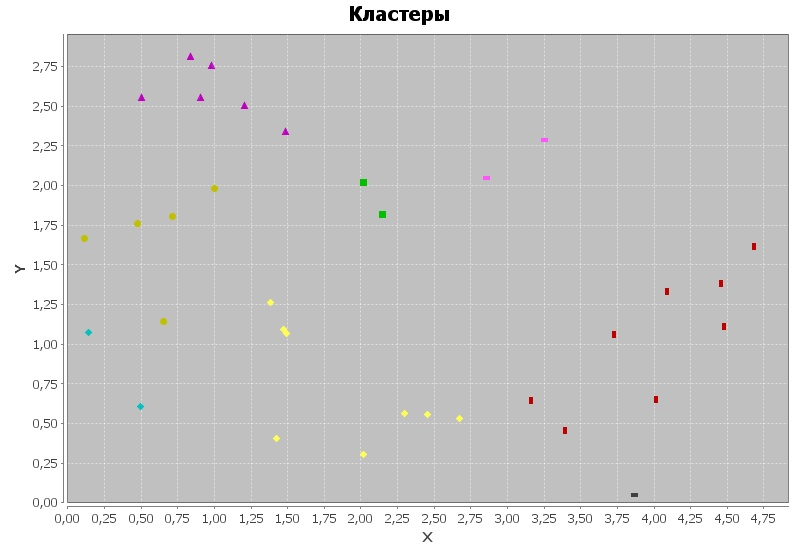
\includegraphics[scale=0.8]{figure_1.png}
	\caption{Результат применения метода ближайшего соседа}
	\label{fig:im_1}
	\end{figure}
\end{center}

\newpage\section{Метод k-средних}
Этот метод является наиболее популярным методом кластеризации, но обладает существенным недостатком: необходимо заранее знать количество искомых кластеров. Обычно для этого используют либо другие методы кластерного анализа, либо какие-то экспериментальные или интуитивные значения.

\vspace{0.5cm}
Суть алгоритма в том, что он стремится минимизировать суммарное квадратичное отклонение точек кластеров от центров этих кластеров. Множество элементов разбивается на заранее известное число кластеров случайным образом. На каждой итерации перевычисляется "центр масс" для каждого кластера, полученного на предыдущем шаге, затем элементы заново разбиваются на кластеры в соответствии с тем, какой из новых центров оказался ближе по выбранной метрике.

\vspace{0.5cm}
Алгоритм завершается, когда на какой-то итерации не происходит изменения центра масс кластеров. Это происходит за конечное число итераций, так как количество возможных разбиений конечного множества конечно, а на каждом шаге суммарное квадратичное отклонение не увеличивается, поэтому зацикливание невозможно.

\vspace{0.5cm}
Количество кластеров было взято 12(сколько было полученно предыдущим методом). Результат несколько отличается от полученного ранее(рис. ~\ref{fig:im_2}), это можно объяснить равномерностью расперделения точек. Границы между классами видны, но может быть подобраны не лучшим образом, присутствуют довольно большие и довольно маленькие классы. Тут можно сказать, что качество разбиения зависит от начальных центров кластеров и их количества.

\begin{center}
	\begin{figure}[h]
	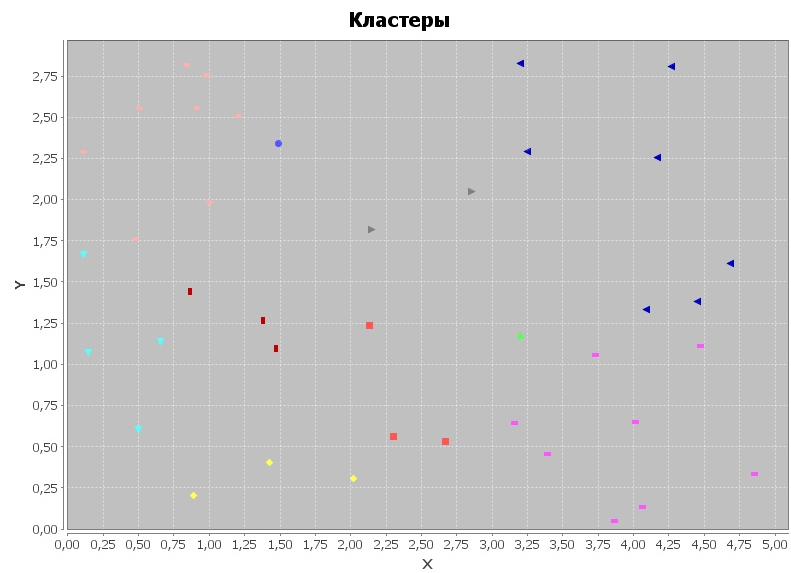
\includegraphics[scale=0.8]{figure_2.png}
	\caption{Результат применения метода k-средних}
	\label{fig:im_2}
	\end{figure}
\end{center}

\newpage\section{Выводы}
Результаты, полученные при помощи рассмотренных методов, очень сильно различаются, что вполне очевидн для случая с довольно равномерно распределенными случайными данными. Можно предположить, что при использовании более разнородных данных, к примеру, массива точек с ярко выраженными скоплениями, результаты были бы более похожими друг на друга. Тем не менее, в обоих случаях задача кластерного анализа была решена и получены ответы, адекватно отвечающие задаче разбиения элементов на классы.


\end{document}